\documentclass{beamer}
\usepackage[utf8]{inputenc}
\usepackage{graphicx, epsfig}
\usepackage{amsmath,mathrsfs,amsfonts,amssymb}
\usepackage{floatflt}
\usepackage{epic,ecltree}
\usepackage{mathtext}
\usepackage{fancybox}
\usepackage{fancyhdr}
\usepackage{multirow}
\usepackage{enumerate}
\usepackage{epstopdf}
\usepackage{multicol}
\usepackage{algorithm}
\usepackage[noend]{algorithmic}
\usepackage{tikz}
\usepackage{blindtext}
\usetheme{default}%{Singapore}%{Warsaw}%{Warsaw}%{Darmstadt}
\usecolortheme{default}

\setbeamerfont{title}{size=\Huge}
\setbeamertemplate{footline}[page number]{}

\setbeamertemplate{section in toc}[sections numbered]


\makeatletter
\newcommand\HUGE{\@setfontsize\Huge{35}{40}}
\makeatother    

\setbeamerfont{title}{size=\HUGE}
\beamertemplatenavigationsymbolsempty

% latin bold lower
\newcommand{\ba}{\mathbf{a}} 
\newcommand{\bc}{\mathbf{c}} 
\newcommand{\be}{\mathbf{e}} 
\newcommand{\bff}{\mathbf{f}} % \bf - for bold type
\newcommand{\bg}{\mathbf{g}} 
\newcommand{\bh}{\mathbf{h}} 
\newcommand{\bp}{\mathbf{p}} 
\newcommand{\bq}{\mathbf{q}} 
\newcommand{\bt}{\mathbf{t}} 
\newcommand{\bs}{\mathbf{s}} 
\newcommand{\bu}{\mathbf{u}} 
\newcommand{\bv}{\mathbf{v}} 
\newcommand{\bw}{\mathbf{w}} 
\newcommand{\bx}{\mathbf{x}} 
\newcommand{\by}{\mathbf{y}} 
\newcommand{\bz}{\mathbf{z}} 

% latin bold upper
\newcommand{\bA}{\mathbf{A}} 
\newcommand{\bB}{\mathbf{B}} 
\newcommand{\bC}{\mathbf{C}} 
\newcommand{\bG}{\mathbf{G}} 
\newcommand{\bI}{\mathbf{I}} 
\newcommand{\bJ}{\mathbf{J}} 
\newcommand{\bL}{\mathbf{L}} 
\newcommand{\bM}{\mathbf{M}} 
\newcommand{\bP}{\mathbf{P}}
\newcommand{\bQ}{\mathbf{Q}} 
\newcommand{\bR}{\mathbf{R}} 
\newcommand{\bT}{\mathbf{T}} 
\newcommand{\bU}{\mathbf{U}} 
\newcommand{\bV}{\mathbf{V}} 
\newcommand{\bW}{\mathbf{W}} 
\newcommand{\bX}{\mathbf{X}} 
\newcommand{\bY}{\mathbf{Y}} 
\newcommand{\bZ}{\mathbf{Z}} 

% latin cal upper
\newcommand{\cF}{\mathcal{F}} 
\newcommand{\cG}{\mathcal{G}} 
\newcommand{\cI}{\mathcal{I}} 
\newcommand{\cL}{\mathcal{L}} 
\newcommand{\cM}{\mathcal{M}} 
\newcommand{\cN}{\mathcal{N}} 
\newcommand{\cP}{\mathcal{P}} 
\newcommand{\cS}{\mathcal{S}} 
\newcommand{\cT}{\mathcal{T}} 
\newcommand{\cW}{\mathcal{W}} 
\newcommand{\cX}{\mathcal{X}} 
\newcommand{\cZ}{\mathcal{Z}} 

% latin bb upper
\newcommand{\bbE}{\mathbb{E}} 
\newcommand{\bbI}{\mathbb{I}} 
\newcommand{\bbP}{\mathbb{P}} 
\newcommand{\bbR}{\mathbb{R}} 

% greek bold lower
\newcommand{\bepsilon}{\boldsymbol{\epsilon}} 
\newcommand{\btheta}{\boldsymbol{\theta}} 
\newcommand{\blambda}{\boldsymbol{\lambda}} 
\newcommand{\bpi}{\boldsymbol{\pi}} 
\newcommand{\bmu}{\boldsymbol{\mu}} 
\newcommand{\bsigma}{\boldsymbol{\sigma}} 
\newcommand{\bphi}{\boldsymbol{\phi}} 

% greek bold upper
\newcommand{\bSigma}{\boldsymbol{\Sigma}} 

\DeclareMathOperator*{\argmin}{arg\,min}
\DeclareMathOperator*{\argmax}{arg\,max}

\newcommand{\createdgmtitle}[1]{\title[\hbox to 56mm{Deep Generative Models  \hfill\insertframenumber\,/\,\inserttotalframenumber}]
	{\vspace{1cm} \\ \textbf{Deep Generative Models} \\ {\Huge Lecture #1}}
	\author{Roman Isachenko}
		\institute{
\includegraphics[width=0.7cm]{../utils/aimasterslogo} \LARGE{AI Masters}}
	\date{2024, Spring}
}

\usepackage{tikz}
\usetikzlibrary{arrows,shapes,positioning,shadows,trees}

\newcommand\myfootnote[1]{%
  \tikz[remember picture,overlay]
  \draw (current page.south west) +(1in + \oddsidemargin,0.5em)
  node[anchor=south west,inner sep=0pt]{\parbox{\textwidth}{%
      \rlap{\rule{10em}{0.4pt}}\raggedright\scriptsize \textit{#1}}};}

\newcommand\myfootnotewithlink[2]{%
  \tikz[remember picture,overlay]
  \draw (current page.south west) +(1in + \oddsidemargin,0.5em)
  node[anchor=south west,inner sep=0pt]{\parbox{\textwidth}{%
      \rlap{\rule{10em}{0.4pt}}\raggedright\scriptsize\href{#1}{\textit{#2}}}};}
      
\AtBeginSection[]
      {
      	\begin{frame}{Outline}
      		\tableofcontents[currentsection]
      	\end{frame}
      }
      \AtBeginSubsection[]{
      	\begin{frame}{Outline}
      		\tableofcontents[currentsection,currentsubsection]
      	\end{frame}
}
\createdgmtitle{10}

\usepackage{tikz}

\usetikzlibrary{arrows,shapes,positioning,shadows,trees}
%--------------------------------------------------------------------------------
\begin{document}
%--------------------------------------------------------------------------------
\begin{frame}[noframenumbering,plain]
%\thispagestyle{empty}
\titlepage
\end{frame}
%=======
\begin{frame}{Recap of previous lecture}
	\vspace{-0.3cm}
	\begin{figure}
		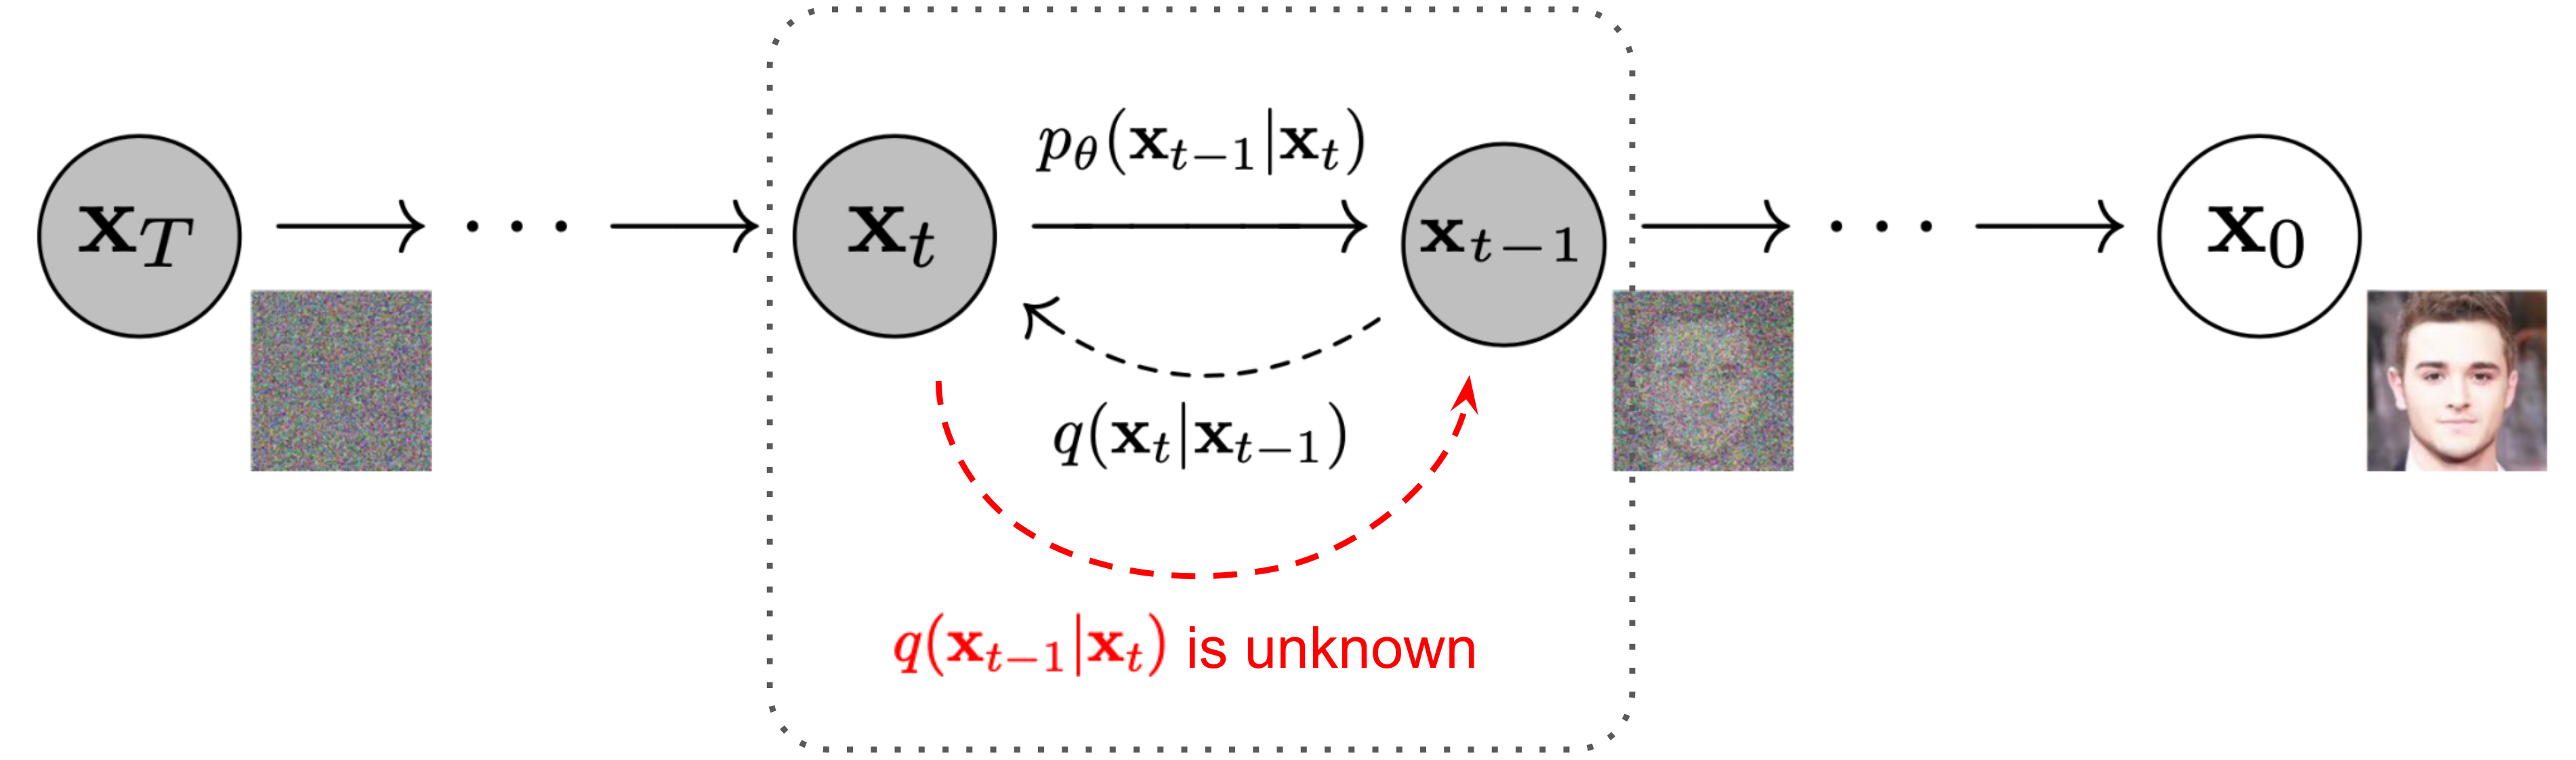
\includegraphics[width=0.8\linewidth]{figs/DDPM}
	\end{figure}
	\vspace{-0.5cm}
	\begin{block}{Reverse process}
		\vspace{-0.5cm}
		{\small
		\[
			q(\bx_{t-1}|\bx_{t}) = \frac{q(\bx_{t}|\bx_{t-1}) {\color{violet}q(\bx_{t-1})}}{{\color{violet}q(\bx_{t})}} \approx p(\bx_{t - 1} | \bx_t, \btheta) = \cN \left(\bmu_{\btheta, t}(\bx_t), \bsigma_{\btheta, t}^2(\bx_t)\right)
		\]}
		{\color{gray}Feller theorem shows that it is a reasonable assumption.}
	\end{block}
	\begin{minipage}{0.5\linewidth}
		\begin{block}{Forward process}
			\begin{enumerate}
				\item $\bx_0 = \bx \sim \pi(\bx)$;
				\item $\bx_t = \sqrt{1 - \beta_t} \cdot \bx_{t - 1} + \sqrt{\beta_t} \cdot \bepsilon$;
				\item $\bx_T \sim p_{\infty}(\bx) = \cN(0, \bI)$.
			\end{enumerate}
		\end{block}
	\end{minipage}%
	\begin{minipage}{0.55\linewidth}
		\begin{block}{Reverse process}
			\begin{enumerate}
				\item $\bx_T \sim p_{\infty}(\bx) = \cN(0, \bI)$;
				\item $\bx_{t - 1} = \bsigma_{\btheta, t}(\bx_t) \cdot \bepsilon + \bmu_{\btheta, t}(\bx_t)$;
				\item $\bx_0 = \bx \sim \pi(\bx)$;
			\end{enumerate}
		\end{block}
	\end{minipage}
	\myfootnotewithlink{https://lilianweng.github.io/posts/2021-07-11-diffusion-models/}{Weng L. What are Diffusion Models?, blog post, 2021}
\end{frame}
%=======
\begin{frame}{Recap of previous lecture}
	\textbf{Forward process} goes from any distribution $\pi(\bx)$ to $\cN(0, \bI)$ via noise injection.
	\begin{align*}
		q(\bx_t | \bx_{t-1}) &= \cN(\sqrt{1 - \beta_t} \cdot \bx_{t-1}, \beta_t \cdot \bI); \\
		q(\bx_t | \bx_0) &= \cN(\sqrt{\bar{\alpha}_t} \cdot \bx_0, (1 - \bar{\alpha}_t) \cdot \bI).
	\end{align*}
	\textbf{Reverse process} is Intractable distribution that is able to be approximated by Normal (with unknown parameters) for small $\beta_t$.
	\[
		q(\bx_{t-1}|\bx_{t}) = \frac{q(\bx_{t}|\bx_{t-1}) q(\bx_{t-1})}{q(\bx_{t})} \approx \cN \left(\bmu_{\btheta, t}(\bx_t), \bsigma_{\btheta, t}^2(\bx_t)\right)
	\]
	\textbf{Conditioned reverse process} is Normal with the known parameters, which defines how to denoise a noisy image $\bx_t$ with access to what the final, completely denoised image $\bx_0$ should be.
	\[
		q(\bx_{t-1}|\bx_{t}, {\color{olive}\bx_0}) = \cN(\tilde{\bmu}_t(\bx_t, \bx_0), \tilde{\beta}_t \cdot \bI)
	\]
	\myfootnotewithlink{https://arxiv.org/abs/2006.11239}{Ho J. Denoising Diffusion Probabilistic Models, 2020}
\end{frame}
%=======
\begin{frame}{Recap of previous lecture}
	\begin{itemize}
		\item $\bz = (\bx_1, \dots, \bx_T)$ is a latent variable.
		\item Variational posterior distribution
		\vspace{-0.2cm}
		\[
			q(\bz | \bx) = q(\bx_1, \dots, \bx_T | \bx_0) = \prod_{t = 1}^T q(\bx_t | \bx_{t - 1}).
		\]
		\vspace{-0.3cm}
		\item Generative distribution and prior
		\vspace{-0.2cm}
		\[
			p(\bx | \bz, \btheta) = p(\bx_0 | \bx_1, \btheta); \quad 
			p(\bz | \btheta) = \prod_{t=2}^T p(\bx_{t - 1} | \bx_t, \btheta) \cdot p(\bx_T)
		\]
	\end{itemize}
	\vspace{-0.2cm}
	\begin{block}{ELBO}
		\vspace{-0.2cm}
		\[
			\log p(\bx | \btheta) \geq \bbE_{q({\color{teal}\bz} | \bx)} \log \frac{p(\bx, {\color{teal}\bz} | \btheta)}{q({\color{teal}\bz} | \bx)} = \cL_{\bphi, \btheta}(\bx) \rightarrow \max_{q, \btheta}
		\]
		\vspace{-0.5cm}
		\begin{multline*}
			\cL_{\bphi, \btheta}(\bx) =  {\color{olive}\bbE_{q(\bx_1 | \bx_0)} \log p(\bx_0 | \bx_1, \btheta)} - {\color{violet}KL\bigl(q(\bx_T | \bx_0) || p(\bx_T)\bigr)} - \\
			- \sum_{t=2}^T  \underbrace{ \bbE_{q(\bx_t | \bx_0)}KL \bigl(q(\bx_{t-1} | \bx_t, \bx_0) || p(\bx_{t - 1} | \bx_t, \btheta )\bigr)}_{\cL_t}
		\end{multline*}
	\end{block}
	\myfootnotewithlink{https://ayandas.me/blog-tut/2021/12/04/diffusion-prob-models.html}{Das A. An introduction to Diffusion Probabilistic Models, blog post, 2021}
\end{frame}
%=======
\begin{frame}{Recap of previous lecture}
	\begin{block}{ELBO of Gaussian diffusion model}
		\vspace{-0.7cm}
		\begin{multline*}
			\cL_{\bphi, \btheta}(\bx) =  {\color{olive}\bbE_{q(\bx_1 | \bx_0)} \log p(\bx_0 | \bx_1, \btheta)} - {\color{violet}KL\bigl(q(\bx_T | \bx_0) || p(\bx_T)\bigr)} - \\
			- \sum_{t=2}^T  \underbrace{ \bbE_{q(\bx_t | \bx_0)}KL \bigl(q(\bx_{t-1} | \bx_t, \bx_0) || p(\bx_{t - 1} | \bx_t, \btheta )\bigr)}_{\cL_t}
		\end{multline*}
		\vspace{-1.0cm}
	\end{block}
	\begin{align*}
		q(\bx_{t-1} | \bx_t, \bx_0) &= \cN(\tilde{\bmu}_t(\bx_t, \bx_0), \tilde{\beta}_t \bI), \\
		p(\bx_{t - 1} | \bx_t, \btheta) &= \cN \bigl(\bmu_{\btheta, t}(\bx_t), {\color{violet}\bsigma_{\btheta, t}^2(\bx_t)}\bigr)
	\end{align*}
	Our assumption:	${\color{violet}\bsigma_{\btheta, t}^2(\bx_t) = \tilde{\beta}_t \bI}$.
	\[
		\cL_t = \bbE_{q(\bx_t | \bx_0)} \left[\frac{1}{2\tilde{\beta}_t} \bigl\| \tilde{\bmu}_t(\bx_t, \bx_0) - \bmu_{\btheta, t}(\bx_t) \bigr\|^2  \right]
	\]
	\myfootnotewithlink{https://arxiv.org/abs/2006.11239}{Ho J. Denoising Diffusion Probabilistic Models, 2020}
\end{frame}
%=======
\begin{frame}{Recap of previous lecture}
	\begin{block}{Training}
		\begin{enumerate}
			\item Get the sample $\bx_0 \sim \pi(\bx)$.
			\item Get noisy image $\bx_t = \sqrt{\bar{\alpha}_t} \cdot \bx_0 + \sqrt{1 - \bar{\alpha}_t} \cdot \bepsilon$, where $\bepsilon \sim \cN(0, \bI)$.
			\item Compute ELBO 
			\vspace{-0.3cm}
			\begin{multline*}
				\cL_{\bphi, \btheta}(\bx) =  {\color{olive}\bbE_{q(\bx_1 | \bx_0)} \log p(\bx_0 | \bx_1, \btheta)} - {\color{violet}KL\bigl(q(\bx_T | \bx_0) || p(\bx_T)\bigr)} - \\
				- {\color{teal}\sum_{t=2}^T \underbrace{ \bbE_{q(\bx_t | \bx_0)} \left[\frac{1}{2\tilde{\beta}_t} \bigl\| \tilde{\bmu}_t(\bx_t, \bx_0) - \bmu_{\btheta, t}(\bx_t) \bigr\|^2  \right]}_{\cL_t}}
			\end{multline*}
			\vspace{-0.7cm}
		\end{enumerate}
	\end{block}
	\begin{block}{Sampling}
		\begin{enumerate}
			\item Sample $\bx_T \sim \cN(0, \bI)$.
			\item Get denoised image $\bx_{t - 1} = \bmu_{\btheta, t}(\bx_t) +  \sqrt{\tilde{\beta}_t} \cdot \bepsilon$, where $\bepsilon \sim \cN(0, \bI)$.
		\end{enumerate}
	\end{block}
	
	\myfootnotewithlink{https://arxiv.org/abs/2006.11239}{Ho J. Denoising Diffusion Probabilistic Models, 2020}
\end{frame}
%=======
\begin{frame}{Outline}
	\tableofcontents
\end{frame}
%=======
\section{Denoising Diffusion Probabilistic Model (DDPM)}
%=======
\subsection{Reparametrization}
%=======
\begin{frame}{Reparametrization of DDPM}
	\[
		\cL_t = \bbE_{q(\bx_t | \bx_0)} \left[\frac{1}{2\tilde{\beta}_t} \bigl\| \tilde{\bmu}_t(\bx_t, \bx_0) - \bmu_{\btheta, t}(\bx_t) \bigr\|^2  \right]
	\]
	\[
		\tilde{\bmu}_t(\bx_t, \bx_0) = \frac{\sqrt{\alpha_t}(1 - \bar{\alpha}_{t-1})}{1 - \bar{\alpha}_t} \cdot \bx_t + \frac{\sqrt{\bar{\alpha}_{t-1}}(1 - \alpha_t)}{1 - \bar{\alpha}_t} \cdot {\color{olive} \bx_0}
	\]
	\vspace{-0.2cm}
	\[
		\bx_t = \sqrt{\bar{\alpha}_t} \cdot \bx_0 + \sqrt{1 - \bar{\alpha}_t} \cdot \bepsilon \quad \Rightarrow \quad {\color{olive} \bx_0} = \frac{\bx_t -  \sqrt{1 - \bar{\alpha}_t} \cdot \bepsilon}{\sqrt{\bar{\alpha}_t}}
	\]
	\vspace{-0.3cm}
	\begin{itemize}
	\item There is linear dependence between $\bepsilon$, $\bx_t$, $\bx_0$.
	\item Let try to rewrite this mean in terms of $\bx_t$ and $\bepsilon$.
	\end{itemize}
	\vspace{-0.2cm}
	\begin{align*}
		\tilde{\bmu}_t(\bx_t, \bepsilon) &= \frac{\sqrt{\alpha_t}(1 - \bar{\alpha}_{t-1})}{1 - \bar{\alpha}_t} \cdot \bx_t + \frac{\sqrt{\bar{\alpha}_{t-1}}(1 - \alpha_t)}{1 - \bar{\alpha}_t} \cdot {\color{olive} \left(\frac{\bx_t -  \sqrt{1 - \bar{\alpha}_t} \cdot \bepsilon}{\sqrt{\bar{\alpha}_t}}\right)} \\
		&= \frac{1}{\sqrt{\alpha_t}} \cdot \bx_t - \frac{1 - \alpha_t}{\sqrt{\alpha_t (1 - \bar{\alpha}_t)}} \cdot \bepsilon
	\end{align*}
	\myfootnotewithlink{https://arxiv.org/abs/2006.11239}{Ho J. Denoising Diffusion Probabilistic Models, 2020}
	\end{frame}
%=======
\begin{frame}{Reparametrization of DDPM}
	\vspace{-0.3cm}
	\[
		\cL_t = \bbE_{\color{violet}q(\bx_t | \bx_0)} \left[ {\color{olive}\frac{1}{2\tilde{\beta}_t}} \bigl\| \tilde{\bmu}_t(\bx_t, \bx_0) - \bmu_{\btheta, t}(\bx_t) \bigr\|^2  \right]
	\]
	\vspace{-0.3cm}
	\begin{block}{Reparametrization}
		\vspace{-0.7cm}
		\begin{align*}
			\tilde{\bmu}_t(\bx_t, \bx_0) &= \frac{1}{\sqrt{\alpha_t}} \cdot \bx_t - \frac{1 - \alpha_t}{\sqrt{\alpha_t (1 - \bar{\alpha}_t)}} \cdot \bepsilon \\
			\bmu_{\btheta, t}(\bx_t) &= \frac{1}{\sqrt{\alpha_t}} \cdot \bx_t - {\color{teal}\frac{1 - \alpha_t}{\sqrt{\alpha_t (1 - \bar{\alpha}_t)}}} \cdot \bepsilon_{\btheta, t}(\bx_t)
		\end{align*}
		\vspace{-0.7cm}
	\end{block}
		\vspace{-0.5cm}
		\begin{align*}
			\cL_t &=  \bbE_{\color{violet} \bepsilon \sim \cN(0, \bI)} \left[ \frac{{\color{teal}(1 - \alpha_t)^2}}{{\color{olive}2\tilde{\beta}_t} {\color{teal} \alpha_t (1 - \bar{\alpha}_t)}} \bigl\| \bepsilon - \bepsilon_{\btheta, t}({\color{violet}\bx_t}) \bigr\|^2 \right] \\
			& =	 \bbE_{\color{violet}\bepsilon \sim \cN(0, \bI)} \left[ \frac{(1 - \alpha_t)^2}{2\tilde{\beta}_t \alpha_t (1 - \bar{\alpha}_t)} \Bigl\| \bepsilon - \bepsilon_{\btheta, t}\bigl( {\color{violet}\sqrt{\bar{\alpha}_t} \bx_0 + \sqrt{1 - \bar{\alpha}_t} \bepsilon}\bigr) \Bigr\|^2 \right]
		\end{align*}
		At each step of the reverse diffusion process we try to predict the noise~$\bepsilon$ that we used in the forward diffusion process!
	\myfootnotewithlink{https://arxiv.org/abs/2006.11239}{Ho J. Denoising Diffusion Probabilistic Models, 2020}
	\end{frame}
%=======
\begin{frame}{Reparametrization of DDPM}
	\begin{multline*}
		\cL_{\bphi, \btheta}(\bx) =  {\color{olive}\bbE_{q(\bx_1 | \bx_0)} \log p(\bx_0 | \bx_1, \btheta)} - {\color{violet}KL\bigl(q(\bx_T | \bx_0) || p(\bx_T)\bigr)} - \\
		- \sum_{t=2}^T \underbrace{ \bbE_{q(\bx_t | \bx_0)} KL \bigl(q(\bx_{t-1} | \bx_t, \bx_0) || p(\bx_{t - 1} | \bx_t, \btheta )\bigr)}_{\cL_t}
	\end{multline*}
	\vspace{-0.3cm}
	\[
		\cL_t  = \bbE_{\bepsilon \sim \cN(0, \bI)} \left[ \frac{(1 - \alpha_t)^2}{2\tilde{\beta}_t \alpha_t (1 - \bar{\alpha}_t)} \Bigl\| \bepsilon - \bepsilon_{\btheta, t}\bigl( \sqrt{\bar{\alpha}_t} \bx_0 + \sqrt{1 - \bar{\alpha}_t} \bepsilon\bigr) \Bigr\|^2 \right]
	\]
	Let drop the scaling coefficient.
	\begin{block}{Simplified objective}
		\vspace{-0.3cm}
		\[
			 \cL_{\text{simple}} = \bbE_{t \sim U\{2, T\}} \bbE_{\bepsilon \sim \cN(0, \bI)} \Bigl\| \bepsilon - \bepsilon_{\btheta, t}\bigl( \sqrt{\bar{\alpha}_t} \cdot \bx_0 + \sqrt{1 - \bar{\alpha}_t} \cdot \bepsilon\bigr) \Bigr\|^2 
		\]
	\end{block}
	\myfootnotewithlink{https://arxiv.org/abs/2006.11239}{Ho J. Denoising Diffusion Probabilistic Models, 2020}
	\end{frame}
%=======
\subsection{Overview}
%=======
\begin{frame}{Generative models zoo}
	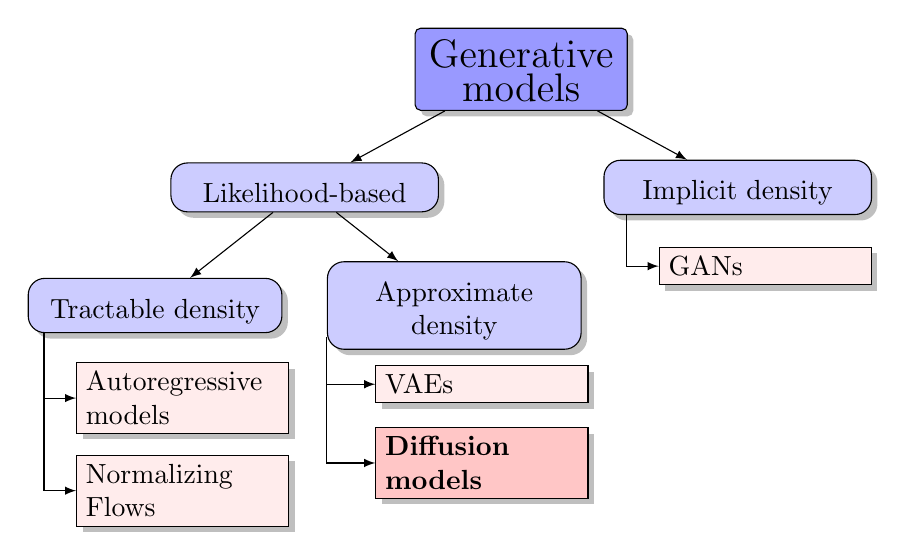
\begin{tikzpicture}[
		basic/.style  = {draw, text width=2cm, drop shadow, rectangle},
		root/.style   = {basic, rounded corners=2pt, thin, text height=1.1em, text width=7em, align=center, fill=blue!40},
		level 1/.style={sibling distance=55mm},
		level 2/.style = {basic, rounded corners=6pt, thin, align=center, fill=blue!20, text height=1.1em, text width=9em, sibling distance=38mm},
		level 3/.style = {basic, rounded corners=6pt, thin,align=center, fill=blue!20, text width=8.5em},
		level 4/.style = {basic, thin, align=left, fill=pink!30, text width=7em},
		level 5/.style = {basic, thin, align=left, fill=pink!90, text width=7em},
		edge from parent/.style={->,draw},
		>=latex]
		
		% root of the the initial tree, level 1
		\node[root] {\Large Generative models}
		% The first level, as children of the initial tree
		child {node[level 2] (c1) {Likelihood-based}
			child {node[level 3] (c11) {Tractable density}}
			child {node[level 3] (c12) {Approximate density}}
		}
		child {node[level 2] (c2) {Implicit density}};
		
		% The second level, relatively positioned nodes
		\begin{scope}[every node/.style={level 4}]
			\node [below of = c11, yshift=-5pt, xshift=10pt] (c111) {Autoregressive models};
			\node [below of = c111, yshift=-5pt] (c112) {Normalizing Flows};
			\node [below of = c12, xshift=10pt] (c121) {VAEs};
			
			\node [below of = c2, xshift=10pt] (c21) {GANs};
		\end{scope}
		
		% The second level, relatively positioned nodes
		\begin{scope}[every node/.style={level 5}]
			\node [below of = c121] (c122) {\textbf{Diffusion \\ models}};
		\end{scope}
		
		% lines from each level 1 node to every one of its "children"
		\foreach \value in {1,2}
		\draw[->] (c11.194) |- (c11\value.west);
		
		\foreach \value in {1,2}
		\draw[->] (c12.194) |- (c12\value.west);
		
		\draw[->] (c2.194) |- (c21.west);
		
	\end{tikzpicture}
\end{frame}
%=======
\begin{frame}{Denoising diffusion probabilistic model (DDPM)}
	\begin{block}{DDPM is a VAE model}
		\begin{itemize}
			\item Encoder is a fixed Gaussian Markov chain $q(\bx_1, \dots, \bx_T | \bx_0)$.
			\item Latent variable is a hierarchical (in each step the dim. of the latent equals to the dim of the input).
			\item Decoder is a simple Gaussian model $p(\bx_0 | \bx_1, \btheta)$.
			\item Prior distribution is given by parametric Gaussian Makov chain $p(\bx_{t-1} | \bx_t, \btheta)$.
		\end{itemize}
	\end{block}
	\begin{minipage}{0.5\linewidth}
		\begin{block}{Forward process}
			\begin{enumerate}
				\item $\bx_0 = \bx \sim \pi(\bx)$;
				\item $\bx_t = \sqrt{1 - \beta_t} \cdot \bx_{t - 1} + \sqrt{\beta_t} \cdot \bepsilon$;
				\item $\bx_T \sim p_{\infty}(\bx) = \cN(0, \bI)$.
			\end{enumerate}
		\end{block}
	\end{minipage}%
	\begin{minipage}{0.55\linewidth}
		\begin{block}{Reverse process}
			\begin{enumerate}
				\item $\bx_T \sim p_{\infty}(\bx) = \cN(0, \bI)$;
				\item $\bx_{t - 1} = \bsigma_{\btheta, t}(\bx_t) \cdot \bepsilon + \bmu_{\btheta, t}(\bx_t)$;
				\item $\bx_0 = \bx \sim \pi(\bx)$;
			\end{enumerate}
		\end{block}
	\end{minipage}
	\myfootnotewithlink{https://arxiv.org/abs/2006.11239}{Ho J. Denoising Diffusion Probabilistic Models, 2020}
\end{frame}
%=======
\begin{frame}{Denoising diffusion probabilistic model (DDPM)}
	\begin{block}{Training}
		\begin{enumerate}
			\item Get the sample $\bx_0 \sim \pi(\bx)$.
			\item Sample timestamp $t \sim U\{1, T\}$ and the noise $\bepsilon \sim \cN(0, \bI)$.
			\item Get noisy image $\bx_t = \sqrt{\bar{\alpha}_t} \cdot \bx_0 + \sqrt{1 - \bar{\alpha}_t} \cdot \bepsilon$.
			\item Compute loss $ \cL_{\text{simple}} = \| \bepsilon - \bepsilon_{\btheta, t}(\bx_t) \|^2 $.
		\end{enumerate}
	\end{block}
	\begin{block}{Sampling (ancestral sampling)}
		\begin{enumerate}
			\item Sample $\bx_T \sim \cN(0, \bI)$.
			\item Compute mean of $p(\bx_{t-1} | \bx_t, \btheta) = \cN(\bmu_{\btheta, t}(\bx_t), \tilde{\beta}_t \cdot \bI)$:
			\[
				\bmu_{\btheta, t}(\bx_t) = \frac{1}{\sqrt{\alpha_t}} \cdot \bx_t - \frac{1 - \alpha_t}{\sqrt{\alpha_t (1 - \bar{\alpha}_t)}} \cdot \bepsilon_{\btheta, t}(\bx_t)
			\]
			\vspace{-0.3cm}
			\item Get denoised image $\bx_{t - 1} = \bmu_{\btheta, t}(\bx_t) +  \sqrt{\tilde{\beta}_t} \cdot \bepsilon$, where $\bepsilon \sim \cN(0, \bI)$.
		\end{enumerate}
	\end{block}
	\myfootnotewithlink{https://arxiv.org/abs/2006.11239}{Ho J. Denoising Diffusion Probabilistic Models, 2020}
\end{frame}
%=======
\begin{frame}{Denoising diffusion probabilistic model (DDPM)}
	\begin{block}{Samples}
		\begin{figure}
			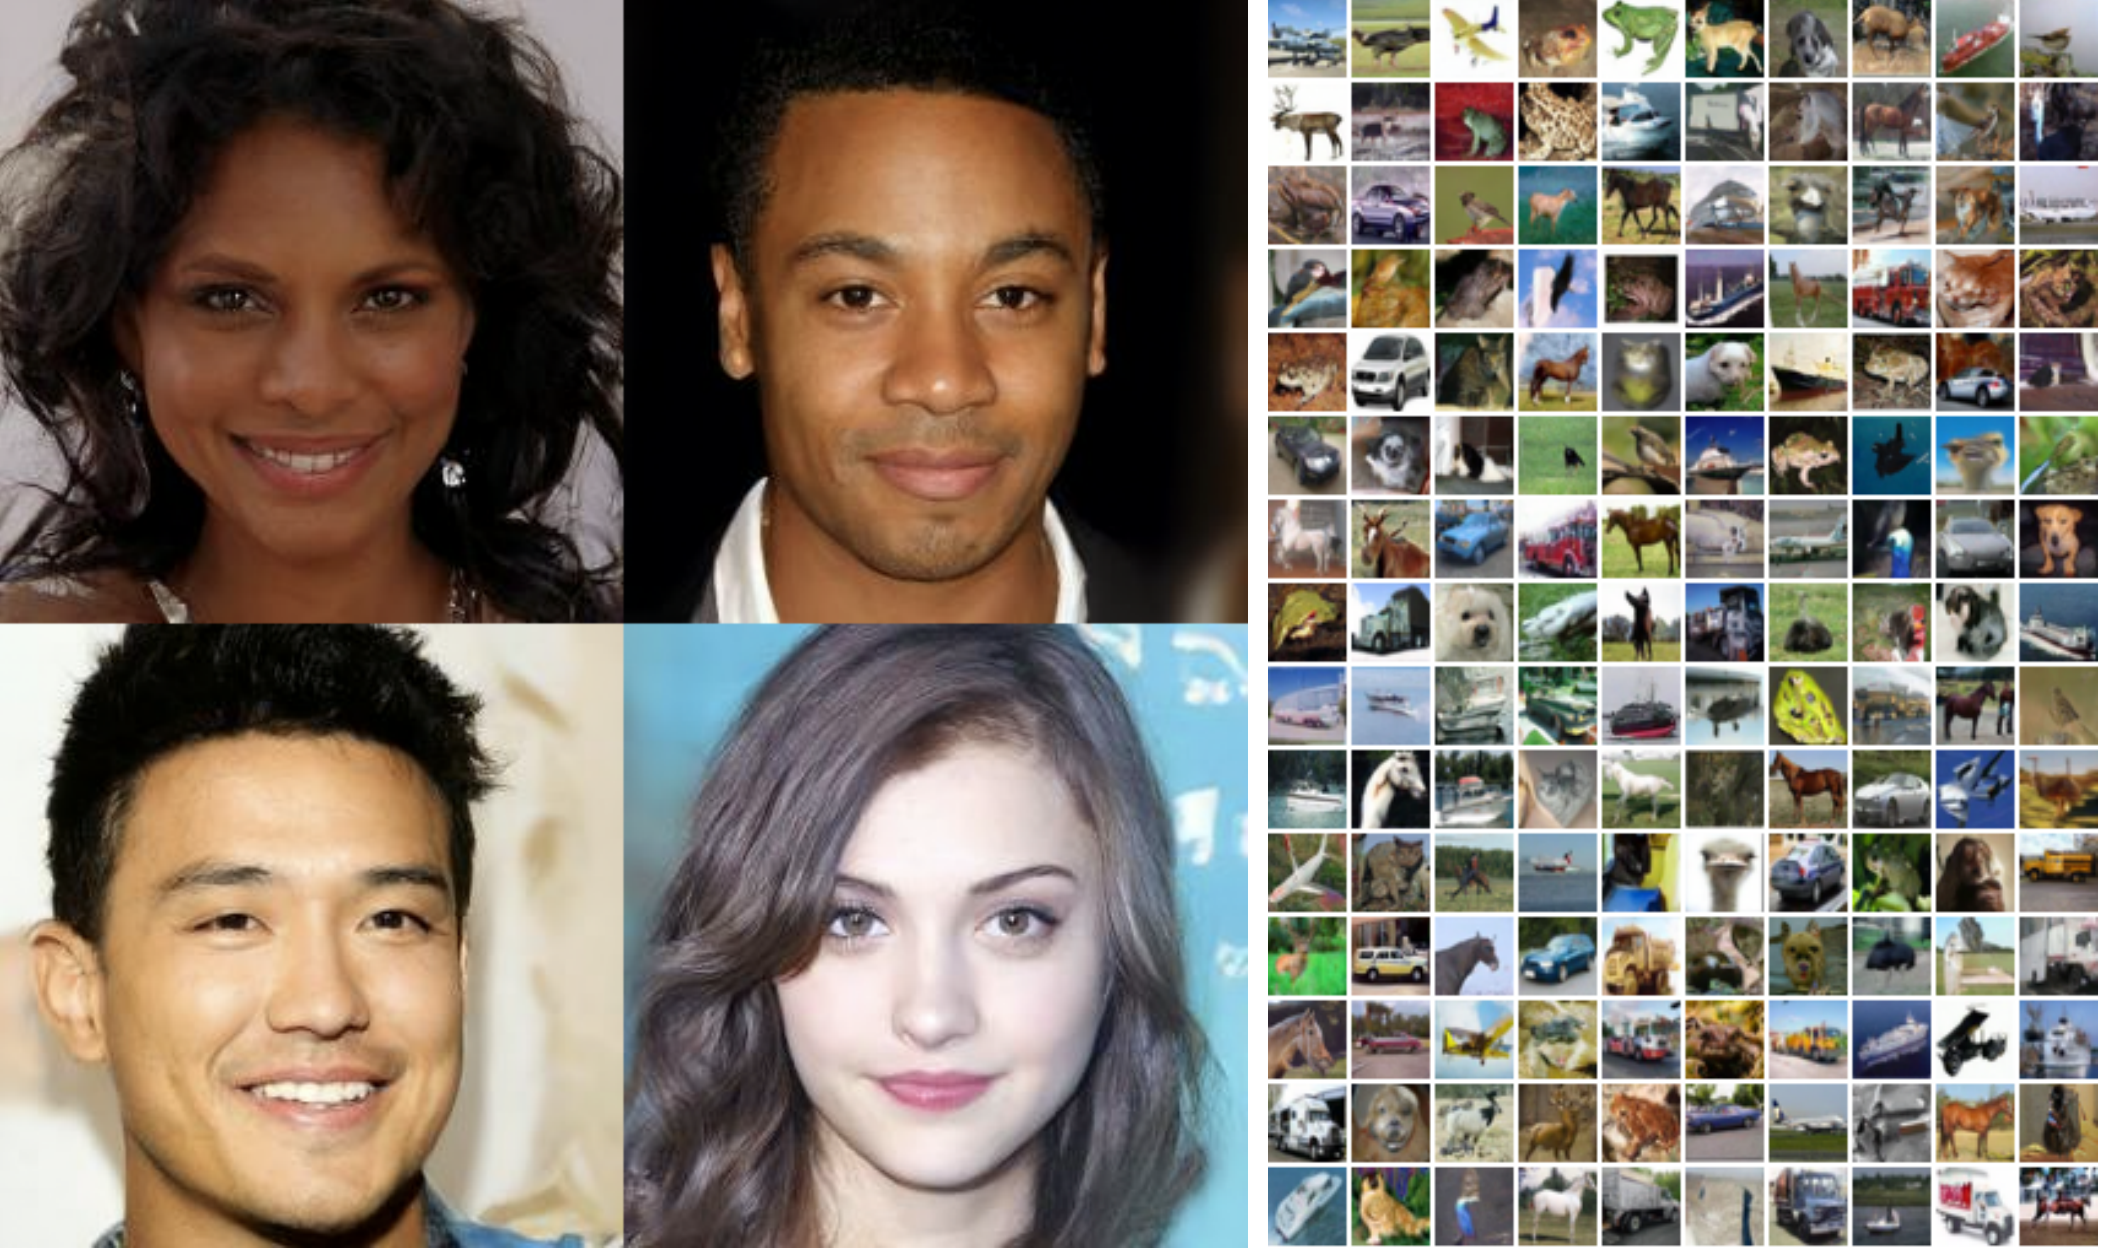
\includegraphics[width=\linewidth]{figs/ddpm_samples}
		\end{figure}
	\end{block}
	\myfootnotewithlink{https://arxiv.org/abs/2006.11239}{Ho J. Denoising Diffusion Probabilistic Models, 2020}
\end{frame}
%=======
\subsection{DDPM as score-based generative model}
%=======
\begin{frame}{Denosing diffusion as score-based generative model}
	\begin{block}{DDPM objective}
		\vspace{-0.7cm}
		\begin{align*}
			\cL_t &= \bbE_{\bepsilon \sim \cN(0, \bI)} \left[ \frac{(1 - \alpha_t)^2}{2\tilde{\beta}_t \alpha_t  (1 - \bar{\alpha}_t)}  \left\|  \bepsilon_{\btheta, t} (\bx_t) - \bepsilon\right\|_2^2  \right] \\
			& = \bbE_{\bepsilon \sim \cN(0, \bI)} \left[ \frac{(1 - \alpha_t)^2}{2\tilde{\beta}_t \alpha_t }  \Bigl\| {\color{violet} \frac{\bepsilon_{\btheta, t}  (\bx_t) }{\sqrt{1 - \bar{\alpha}_t}}} - {\color{teal}\frac{\bepsilon}{\sqrt{1 - \bar{\alpha}_t}}}\Bigr\|_2^2  \right]
		\end{align*}
		\vspace{-0.7cm}
	\end{block}
	\vspace{-0.5cm}
	\begin{align*}
		q(\bx_t | \bx_0) &= \cN(\sqrt{\bar{\alpha}_t} \cdot \bx_0, (1 - \bar{\alpha}_t) \cdot \bI) \\
		\nabla_{\bx_t} \log q(\bx_t | \bx_0) &= - \frac{\bx_t - \sqrt{\bar{\alpha}_t} \cdot \bx_0}{1 - \bar{\alpha}_t} = {\color{teal}-  \frac{\bepsilon}{\sqrt{1 - \bar{\alpha}_t}}}.
	\end{align*}
		Let reparametrize our model: 
		\vspace{-0.2cm}
		\[
			\bs_{\btheta, t}(\bx_t) = {\color{violet}- \frac{\bepsilon_{\btheta, t}(\bx_t)}{\sqrt{1 - \bar{\alpha}_t}}} = \nabla_{\bx_t} \log p(\bx_t | \btheta).
		\]
		\[
			\cL_t = \bbE_{q(\bx_t | \bx_0)} \left[ \frac{(1 - \alpha_t)^2}{2\tilde{\beta}_t \alpha_t}  \Bigl\|  \bs_{\btheta, t} (\bx_t) - \nabla_{\bx_t} \log q(\bx_t | \bx_0) \Bigr\|_2^2  \right]
		\]
	\myfootnotewithlink{https://arxiv.org/abs/2006.11239}{Ho J. Denoising Diffusion Probabilistic Models, 2020}
	\end{frame}
%=======
\begin{frame}{DDPM vs NCSN: objectives}
	\begin{block}{DDPM objective}
		\vspace{-0.5cm}
		\[
			\bbE_{\pi(\bx_0)} \bbE_{t \sim U\{1, T\}}\bbE_{q(\bx_t | \bx_0)} \left[ {\color{olive}\frac{(1 - \alpha_t)^2}{2\tilde{\beta}_t \alpha_t}} \Bigl\|  \bs_{\btheta, t} (\bx_t) - \nabla_{\bx_t} \log q(\bx_t | \bx_0) \Bigr\|_2^2  \right]
		\]
		\[
			\bx_t = \sqrt{\bar{\alpha}_t} \cdot \bx_0 + \sqrt{1 - \bar{\alpha}_t} \cdot \bepsilon
		\]
		In practice {\color{olive}the coefficient} is omitted.
	\end{block}
	\begin{block}{NCSN objective}
		\vspace{-0.3cm}
		\[
			\bbE_{\pi(\bx_0)} \bbE_{t \sim U\{1, T\}} \bbE_{q(\bx_t | \bx_0)}\bigl\| \bs_{\btheta, \sigma_t}(\bx_t) - \nabla_{\bx_t} \log q(\bx_t | \bx_0) \bigr\|^2_2 
		\]
		\[
			\bx_t = \bx_0 + \sigma_t \cdot \bepsilon
		\]
		\vspace{-0.5cm}
	\end{block}
	\textbf{ELBO maximization approach gives the same objective as denoising score-matching approach!}
	\myfootnotewithlink{https://arxiv.org/abs/2006.11239}{Ho J. Denoising Diffusion Probabilistic Models, 2020}
	\end{frame}
%=======
\begin{frame}{DDPM vs NCSN: sampling}
	\begin{block}{DDPM sampling (ancestral sampling)}
			\vspace{-0.7cm}
			\begin{align*}
				\bx_T &\sim \cN(0, \bI) \\
				\bx_{t - 1} &= {\color{teal}\bmu_{\btheta, t}(\bx_t)} + \sigma_t \cdot \bepsilon \\
				& ={\color{teal}\frac{1}{\sqrt{\alpha_t}} \cdot \bx_t - \frac{1 - \alpha_t}{\sqrt{\alpha_t (1 - \bar{\alpha}_t)}} \cdot \bepsilon_{\btheta, t}(\bx_t)} +  \sigma_t \cdot \bepsilon \\
				& = \frac{1}{\sqrt{1 - \beta_t}} \cdot \bx_t + \frac{\beta_t}{\sqrt{1 - \beta_t}} \cdot \bs_{\btheta, t} (\bx_t) +  \sigma_t \cdot \bepsilon
			\end{align*}
			\vspace{-0.5cm}
	\end{block}
	\begin{block}{NCSN sampling (annealed Langevin dynamics)}
		\begin{itemize}
			\item Sample $\bx_T^0 \sim \cN(0, \sigma_T^2 \cdot \bI) \approx q(\bx_T)$.
			\item Apply $L$ steps of Langevin dynamic
			\vspace{-0.2cm}
			\[
				\bx_t^l = \bx_t^{l-1} + \frac{\eta_t}{2} \cdot \bs_{\btheta, \sigma_t}(\bx_t^{l - 1}) + \sqrt{\eta_t} \cdot \bepsilon_t^l.
			\] 
			\vspace{-0.7cm}
			\item Update $\bx_{t-1}^0 = \bx_t^L$ and choose the next $\sigma_t$.
		\end{itemize}
	\end{block}
	\myfootnotewithlink{https://arxiv.org/abs/2006.11239}{Ho J. Denoising Diffusion Probabilistic Models, 2020}
	\end{frame}
%=======
\begin{frame}{DDPM vs NCSN}
	\begin{block}{Summary}
		\begin{itemize}
		\item Different Markov chains:
			\begin{itemize}
				\item DDPM: $\bx_t = \sqrt{\bar{\alpha}_t} \cdot \bx_0 + \sqrt{1 - \bar{\alpha}_t} \cdot \bepsilon$;
				\item NCSN: $\bx_t = \bx_0 + \sigma_t \cdot \bepsilon$.
				\item It is possible to consider the more general framework $q(\bx_t |\bx_0) = \cN(\alpha_t \cdot \bx_0, \sigma^2_t\cdot \bI)$
			\end{itemize}
		\item Identical objectives: ELBO $\equiv$ score-matching.
		\item Different sampling schemes:
			\begin{itemize}
				\item ancestral sampling for DDPM;
				\item annealed Langevin dynamics for NCSN;
				\item there is a combined approach with alternating updates of DDPM and NCSN.
			\end{itemize}
		\end{itemize}
	\end{block}
	\myfootnote{\href{https://arxiv.org/abs/2107.00630}{Kingma D. et al. Variational Diffusion Models, 2021} \\
	\href{}{Song Y. et al. Score-Based Generative Modeling through Stochastic Differential Equations, 2020}}
	\end{frame}
\section{Guidance}
%=======
\begin{frame}{Guidance}
	\begin{itemize}
	\item Throughout the whole course we have discussed unconditional generative models $p(\bx | \btheta)$.
	\item In practice the majority of the generative models are $\textbf{conditional}$: $p(\bx | \by, \btheta)$.
	\item Here $\by$ could be the class label or $\textbf{text}$ (for text-to-image models).
	\end{itemize}
	\vspace{-0.3cm}
	\begin{minipage}[t]{0.5\columnwidth}
		\begin{figure}
			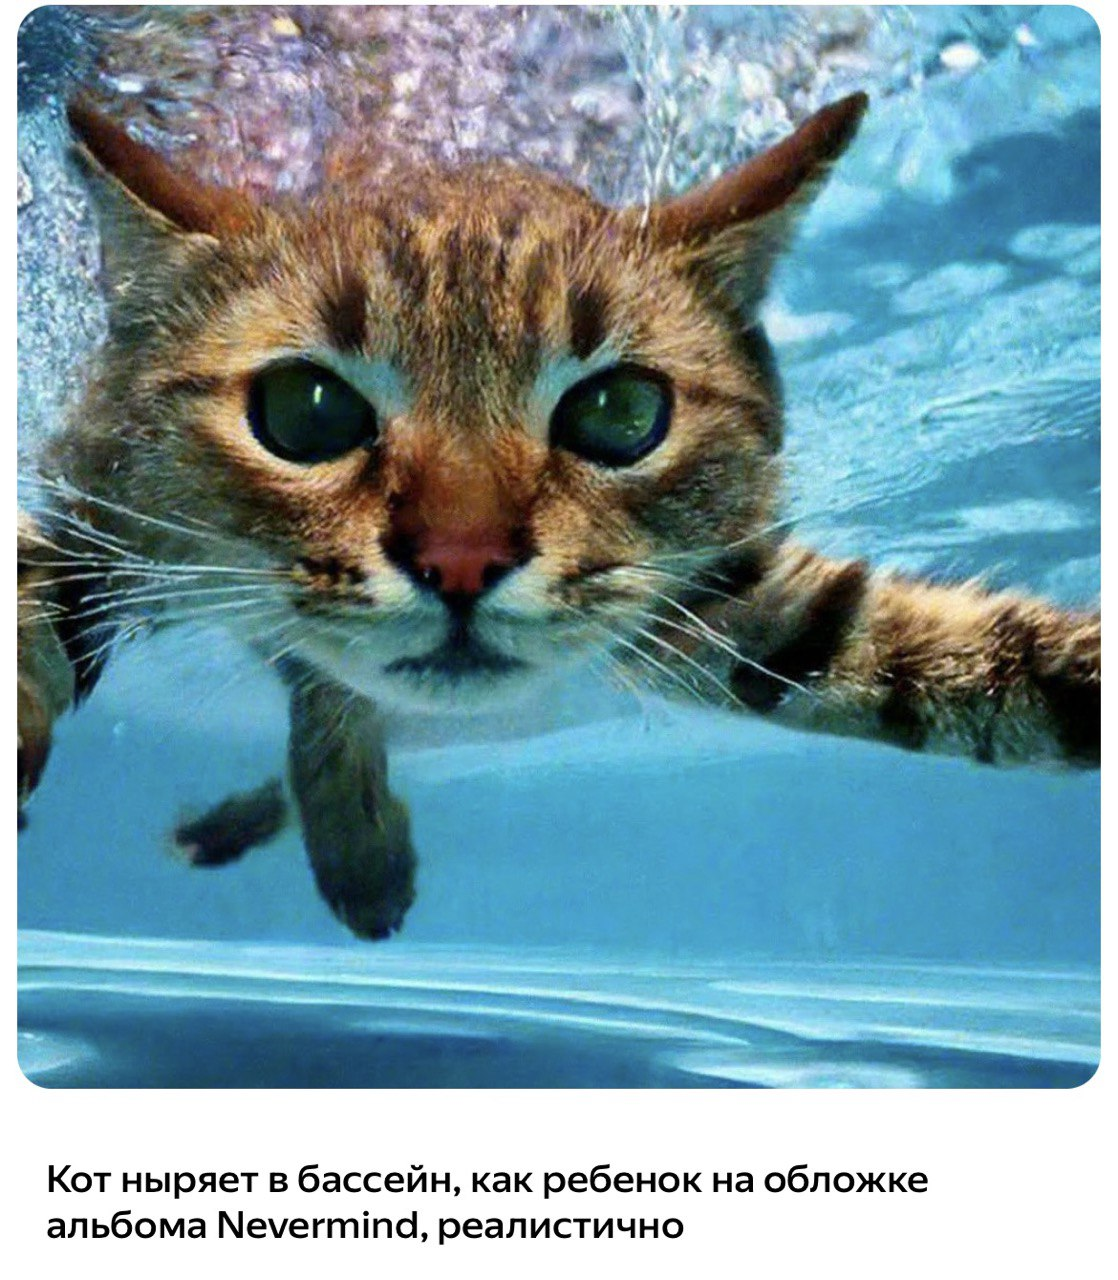
\includegraphics[width=0.9\linewidth]{figs/shedevrum1}
		\end{figure}
	\end{minipage}%
	\begin{minipage}[t]{0.5\columnwidth}
		\begin{figure}
			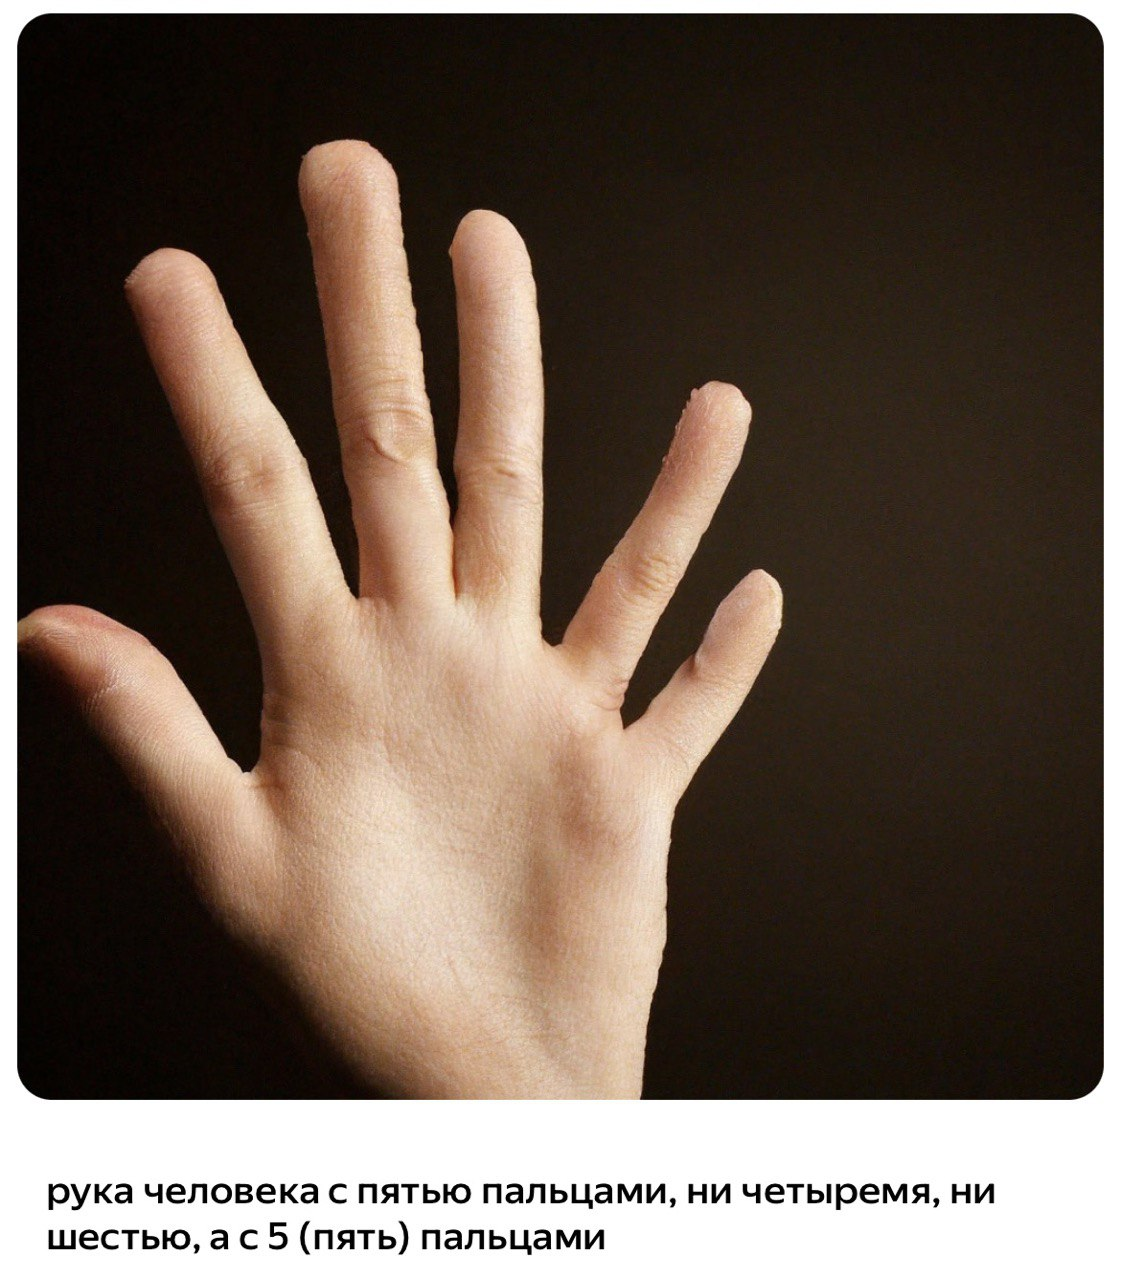
\includegraphics[width=0.9\linewidth]{figs/shedevrum2}
		\end{figure}
	\end{minipage}
\end{frame}
%=======
\begin{frame}{Taxonomy of conditional tasks}
	In practice the popular task is to create a conditional model~$\pi(\bx | \by)$. 
	\begin{itemize}
	\item $\by$ -- class label, $\bx$ -- image $\Rightarrow$ image conditional model.
	\item $\by$ -- text prompt, $\bx$ -- image $\Rightarrow$ text-to-image model.
	\item $\by$ -- image, $\bx$ -- image $\Rightarrow$ image-to-image model.
	\item $\by$ -- image, $\bx$ -- text $\Rightarrow$ image-to-text model (image captioning).
	\item $\by$ -- sound, $\bx$ -- text $\Rightarrow$ speech-to-text model (automatic speech recognition).
	\item $\by$ -- English text, $\bx$ -- Russian text $\Rightarrow$ sequence-to-sequence model (machine translation).
	\item $\by = \emptyset$, $\bx$ -- image $\Rightarrow$ image unconditional model.
	\end{itemize}
\end{frame}
%=======
\begin{frame}{Label guidance}
	\textbf{Label:} Ostrich (10th ImageNet class) 
	\begin{figure}
		\includegraphics[width=\linewidth]{figs/label_conditioning}
	\end{figure}
	\myfootnotewithlink{https://arxiv.org/abs/1906.00446}{Razavi A., Oord A., et al. Generating Diverse High-Fidelity Images with VQ-VAE-2, 2019}\end{frame}
%=======
\begin{frame}{Text guidance}
	\textbf{Prompt:} a stained glass window of a panda eating bamboo \\
	Left: $\gamma = 1$, Right: $\gamma = 3$.
	\begin{figure}
		\includegraphics[width=\linewidth]{figs/cfg}
	\end{figure}
	\myfootnotewithlink{https://arxiv.org/pdf/2112.10741}{Nichol A., et al. GLIDE: Towards Photorealistic Image Generation and Editing with Text-Guided Diffusion Models, 2022}
\end{frame}
%=======
\begin{frame}{Guidance}
	\begin{itemize}
	\item If we have \textbf{supervised} data $\{(\bx_i, \by_i)\}_{i=1}^n$ we could theat $\by$ as additional model input:
	\begin{itemize}
		\item $p(x_j | \bx_{1:j-1}, {\color{olive}\by}, \btheta)$ for AR;
		\item Encoder $q(\bz | \bx, {\color{olive}\by}, \bphi)$ and decoder $p(\bx | \bz, {\color{olive}\by}, \btheta)$ for VAE;
		\item $G_{\btheta}(\bz, {\color{olive}\by})$ for NF and GAN;
		\item $p(\bx_{t-1} | \bx_t, {\color{olive}\by}, \btheta)$ for DDPM.
	\end{itemize}
	\item If we have \textbf{unsupervised} data $\{\bx_i\}_{i=1}^n$ we need to create the way to convert unconditional model $p(\bx | \btheta)$ to the conditional.
	\item It is really helpful to have the way to control the power of guidance.
	\end{itemize}
	\begin{block}{Guidance types}
		\begin{itemize}
			\item \textbf{Classifier guidance:} 
				\begin{itemize}
					\item suitable for unsupervised data;
					\item uses the additional classifier model.
				\end{itemize}
			\item \textbf{Classifier-free guidance:} 
				\begin{itemize}
					\item suitable for supervised data;
					\item get rid of the additional classifier model.
				\end{itemize}
		\end{itemize}
	\end{block}
\end{frame}
%=======
\subsection{Classifier guidance}
%=======
\begin{frame}{Classifier guidance}
	
	\begin{block}{DDPM sampling}
		\begin{enumerate}
			\item Sample $\bx_T \sim \cN(0, \bI)$.
			\item Get denoised image (unconditional generation)
			\vspace{-0.3cm}
			\begin{align*}
				\bx_{t - 1} &= \frac{1}{\sqrt{1 - \beta_t}} \cdot \bx_t + \frac{\beta_t}{\sqrt{1 - \beta_t}} \cdot {\color{teal}\bs_{\btheta, t} (\bx_t)} +  \sigma_t \cdot \bepsilon \\
				& = \frac{1}{\sqrt{1 - \beta_t}} \cdot \bx_t + \frac{\beta_t}{\sqrt{1 - \beta_t}} \cdot {\color{teal} \nabla_{\bx_t} \log p(\bx_t | \btheta)} +  \sigma_t \cdot \bepsilon
			\end{align*}
			\vspace{-0.5cm}
		\end{enumerate}
	\end{block}
	\begin{block}{Conditional generation}
		\vspace{-0.3cm}
		\[
			\bx_{t - 1} = \frac{1}{\sqrt{\alpha_t}} \cdot \bx_t + \frac{1 - \alpha_t}{\sqrt{\alpha_t}} \cdot  \nabla_{\bx_t} \log p(\bx_t | {\color{olive}\by}, \btheta) +  \sigma_t \cdot \bepsilon
		\]
		\vspace{-0.5cm}
	\end{block}
	\begin{itemize}
		\item Assume for simplicity $\by$ is a class labels.
		\item Suppose that we have the distribution $p(\by | \bx_t)$ -- classifier on noisy samples.
	\end{itemize}
	\myfootnotewithlink{https://arxiv.org/abs/2105.05233}{Dhariwal P., Nichol A. Diffusion Models Beat GANs on Image Synthesis, 2021}
\end{frame}
%=======
\begin{frame}{Classifier guidance}
	\begin{block}{Conditional generation}
		\vspace{-0.3cm}
		\[
			\bx_{t - 1} = \frac{1}{\sqrt{\alpha_t}} \cdot \bx_t + \frac{1 - \alpha_t}{\sqrt{\alpha_t}} \cdot  \nabla_{\bx_t} \log p(\bx_t | {\color{olive}\by}, \btheta) +  \sigma_t \cdot \bepsilon
		\]
		\vspace{-0.5cm}
	\end{block}
	\begin{block}{Conditional distribution}
		\vspace{-0.7cm}
		\begin{align*}
			{\color{olive}\nabla_{\bx_t} \log p(\bx_t | \by, \btheta)} &= \nabla_{\bx_t} \log \left(\frac{p(\by | \bx_t)p(\bx_t | \btheta)}{p(\by)} \right)\\
			&= \nabla_{\bx_t} \log p(\by | \bx_t) + {\color{violet}\nabla_{\bx_t} \log p(\bx_t | \btheta)}\\
			&= {\color{teal}\nabla_{\bx_t} \log p(\by | \bx_t)} {\color{violet}- \frac{\bepsilon_{\btheta, t}(\bx_t)}{\sqrt{1 - \bar{\alpha}_t}}}
		\end{align*}
		\vspace{-0.5cm}
	\end{block}
	Let parametetrize $\nabla_{\bx_t} \log p(\bx_t | \by, \btheta) = - \frac{\bepsilon_{\btheta, t}(\bx_t, \by)}{\sqrt{1 - \bar{\alpha}_t}}$.
	\begin{block}{Classifier-corrected noise prediction}
		\vspace{-0.3cm}
		\[
			{\color{olive}\bepsilon_{\btheta, t}(\bx_t, \by)} = {\color{violet}\bepsilon_{\btheta, t}(\bx_t)} - \sqrt{1 - \bar{\alpha}_t} \cdot {\color{teal}\nabla_{\bx_t} \log p(\by | \bx_t)}
		\]
	\end{block}
	\myfootnotewithlink{https://arxiv.org/abs/2105.05233}{Dhariwal P., Nichol A. Diffusion Models Beat GANs on Image Synthesis, 2021}
\end{frame}
%=======
\begin{frame}{Classifier guidance}
	\begin{block}{Classifier-corrected noise prediction}
		\vspace{-0.3cm}
		\[
			\bepsilon_{\btheta, t}(\bx_t, \by) = \bepsilon_{\btheta, t}(\bx_t) - \sqrt{1 - \bar{\alpha}_t} \cdot \nabla_{\bx_t} \log p(\by | \bx_t)
		\]
		\vspace{-0.5cm}
	\end{block}
	\begin{block}{Guidance scale}
		\vspace{-0.3cm}
		\[
			{\color{olive}\bepsilon_{\btheta, t}(\bx_t, \by)} = \bepsilon_{\btheta, t}(\bx_t) - {\color{teal}\gamma} \cdot \sqrt{1 - \bar{\alpha}_t} \cdot \nabla_{\bx_t} \log p(\by | \bx_t)
		\]
		Here we introduce {\color{teal} guidance scale $\gamma$} that controls the magnitude of the classifier guidance.
	\end{block}
	\begin{block}{Training}
		\begin{itemize}
			\item Train DDPM as usual.
			\item Train the additional classifier $p(\by | \bx_t)$ on the noisy samples $\bx_t$.
		\end{itemize}
		\vspace{-0.2cm}
	\end{block}
	\begin{block}{Guided sampling}
		\vspace{-0.3cm}
		\[
			\bx_{t-1} = \frac{1}{\sqrt{\alpha_t}} \cdot \bx_t - \frac{1 - \alpha_t}{\sqrt{\alpha_t (1 - \bar{\alpha}_t)}} \cdot  {\color{olive}\bepsilon_{\btheta, t}(\bx_t, \by)} + \sigma_t \cdot \bepsilon
		\]
	\end{block}
	\myfootnotewithlink{https://arxiv.org/abs/2105.05233}{Dhariwal P., Nichol A. Diffusion Models Beat GANs on Image Synthesis, 2021}
\end{frame}
%=======
\begin{frame}{Classifier guidance}
	\begin{block}{Classifier-corrected noise prediction}
		\vspace{-0.3cm}
		\[
			\bepsilon_{\btheta, t}(\bx_t, \by) = \bepsilon_{\btheta, t}(\bx_t) - {\color{teal}\gamma} \cdot \sqrt{1 - \bar{\alpha}_t} \cdot \nabla_{\bx_t} \log p(\by | \bx_t)
		\]
		\vspace{-0.7cm}
	\end{block}
	\begin{block}{Guidance-scaled conditional distribution}
		\[
			\frac{\bepsilon_{\btheta, t}(\bx_t, \by)}{\sqrt{1 - \bar{\alpha}_t}} = \frac{\bepsilon_{\btheta, t}(\bx_t)}{\sqrt{1 - \bar{\alpha}_t}} - {\color{teal}\gamma} \cdot \nabla_{\bx_t} \log p(\by | \bx_t)
		\]
		\vspace{-0.5cm}
		\begin{align*}
			\nabla_{\bx_t}^{\gamma} \log p(\bx_t | \by, \btheta) &= \nabla_{\bx_t} \log p(\bx_t | \btheta) + \gamma \cdot \nabla_{\bx_t} \log p(\by | \bx_t) \\
			&= \nabla_{\bx_t} \log p(\bx_t | \btheta) + \nabla_{\bx_t} \log p(\by | \bx_t)^{\gamma} \\
			&= \nabla_{\bx_t} \log \left( \frac{p(\by | \bx_t)^{\gamma} p(\bx_t | \btheta)}{Z} \right)
		\end{align*}
		\vspace{-0.5cm}
	\end{block}
	\textbf{Note:} Guidance scale $\gamma$ tries to sharpen the distribution $p(\by | \bx_t)$ (in this case $Z$ should not depend on $\bx_t$).
	\myfootnotewithlink{https://arxiv.org/abs/2105.05233}{Dhariwal P., Nichol A. Diffusion Models Beat GANs on Image Synthesis, 2021}
\end{frame}
%=======
\subsection{Classifier-free guidance}
%=======
\begin{frame}{Classifier-free guidance}
	\begin{itemize}
		\item Previous method requires training the additional classifier model $p(\by | \bx_t)$ on the noisy data.	
		\item Let try to avoid this requirement.
	\end{itemize}
	\[
		\nabla_{\bx_t}^{\gamma} \log p(\bx_t | \by, \btheta) = \nabla_{\bx_t} \log p(\bx_t | \btheta) + \gamma \cdot {\color{teal}\nabla_{\bx_t} \log p(\by | \bx_t)}
	\]
	\vspace{-0.7cm}
	\begin{align*}
		{\color{teal}\nabla_{\bx_t} \log p(\by | \bx_t)} &= \nabla_{\bx_t} \log \left( \frac{p(\bx_t| \by, \btheta) p(\by)}{p(\bx_t | \btheta)} \right) \\
		&=  \nabla_{\bx_t} \log p(\bx_t| \by, \btheta) -\nabla_{\bx_t} \log  p(\bx_t | \btheta)
	\end{align*}
	\vspace{-0.8cm}
	\begin{multline*}
		\nabla_{\bx_t}^{\gamma} \log p(\bx_t | \by, \btheta) = \nabla_{\bx_t} \log p(\bx_t | \btheta) + \gamma \cdot \nabla_{\bx_t} {\color{violet}\log p(\by | \bx_t)} = \\
		= \nabla_{\bx_t} \log p(\bx_t | \btheta) + \gamma \cdot \bigl( {\color{violet}\nabla_{\bx_t} \log p(\bx_t| \by, \btheta) - \nabla_{\bx_t} \log  p(\bx_t | \btheta)} \bigr) = \\
		=  (1 - \gamma) \cdot  \nabla_{\bx_t} \log p(\bx_t | \btheta) + \gamma \cdot  \nabla_{\bx_t} \log p(\bx_t| \by, \btheta)
	\end{multline*}
	\textbf{Note:} In the case of $\gamma = 1$ we will get the identity statement.
	\myfootnotewithlink{https://arxiv.org/abs/2207.12598}{Ho J., Salimans T. Classifier-Free Diffusion Guidance, 2022}
\end{frame}
%=======
\begin{frame}{Classifier-free guidance}
	\[
		\nabla_{\bx_t}^{\gamma} \log p(\bx_t | \by, \btheta) =  (1 - \gamma) \cdot  \nabla_{\bx_t} \log p(\bx_t | \btheta) + \gamma \cdot  \nabla_{\bx_t} \log p(\bx_t| \by, \btheta)
	\]
	\[
		\frac{\bepsilon_{\btheta, t}(\bx_t, \by)}{\sqrt{1 - \bar{\alpha}_t}} = (1 - \gamma) \cdot  \frac{\bepsilon_{\btheta, t}(\bx_t)}{\sqrt{1 - \bar{\alpha}_t}} +  \gamma \cdot \frac{\bepsilon_{\btheta, t}(\bx_t, \by)}{\sqrt{1 - \bar{\alpha}_t}} 
	\]
	\begin{block}{Classifier-free-corrected noise prediction}
		\vspace{-0.3cm}
		\[
			\hat{\bepsilon}_{\btheta, t}(\bx_t, \by) = \gamma \cdot \bepsilon_{\btheta, t}(\bx_t, \by) + (1 - \gamma) \cdot \bepsilon_{\btheta, t}(\bx_t)
		\]
		\vspace{-0.5cm}
	\end{block}
	\begin{itemize}
		\item Train the single model $\bepsilon_{\btheta, t}(\bx_t, \by)$ on \textbf{supervised} data alternating with real conditioning $\by$ and empty conditioning $\by = \emptyset$.
		\item Apply the model twice during inference.
	\end{itemize}
	\myfootnotewithlink{https://arxiv.org/abs/2207.12598}{Ho J., Salimans T. Classifier-Free Diffusion Guidance, 2022}
\end{frame}
%=======
\begin{frame}{Summary}
	\begin{itemize}
		\item At each step DDPM predicts the noise that was used in the forward diffusion process. 
		\vfill
		\item DDPM is a VAE model that tries to invert forward diffusion process using variational inference. 
		\vfill
		\item DDPM is really slow, because we have to apply the model $T$ times.
		\vfill
		\item DDPM and NCSN are closely related in terms of objectives.	
		\vfill
		\item Classifier guidance is the way to turn the unconditional model to the conditional one via the training additional classifier on the noisy data.
		\vfill
		\item Classifier-free guidance allows to avoid the training additional classifier to get the conditional model. It is widely used in practice.
	\end{itemize}
\end{frame}
%=======
\end{document} 